\section*{Tema 1}
\addcontentsline{toc}{section}{Tema 1}
    \subsection*{Conceptos de calidad de Software}
    \addcontentsline{toc}{subsection}{Conceptos de calidad de Software}
        \subsubsection*{¿Qué es la calidad?}
        \addcontentsline{toc}{subsubsection}{¿Qué es la calidad?}
        
            En este curso, entenderemos calidad como "La totalidad de características y atributos de un producto o servicio relacionados con satisfacer necesidades expresas o implícitas". Una definición alternativa es "La medida en que un conjunto de características inherentes satisfacen los requisitos".
            
            Dentro del curso, nos enfocaremos principalmente en la calidad de software y en la calidad de los procesos que rodean a este. A continuación se muestran los principios de calidad de software:
            
            \begin{itemize}
                \item \textbf{Prevenir}
                    Prevenir defectos en vez de corregirlos
                \item \textbf{Detectar temprano}
                    Detectar y corregir defectos lo antes posible
                \item \textbf{Encontrar causas}
                    Determinar y eliminar las causas de los defectos
                \item \textbf{Auditar el trabajo}
                    Auditar el trabajo, en cuanto al uso de procedimientos y estándares
                \item \textbf{Definir}
                    Roles, responsabilidades y procesos
                \item \textbf{Planificar}
                    El trabajo con detalle, a partir de los requerimientos del software
                \item \textbf{Monitorear}
                    Hacer un seguimiento de la ejecución de los planes y tomar medidas correctivas de ser necesario 
                \item \textbf{Refinar}
                    Los planes se deberán refinar a medida que se avanza.
            \end{itemize}
            
            Estos principios deben ser respetados durante cada proyecto.
            
            \newpage
            
            \subsubsection*{Ingeniería de Software}
            \addcontentsline{toc}{subsection}{Ingeniera de Software}
            
            Para introducirnos un poco más, definiremos qué es la Ingeniería de Software. En este curso, se entenderá como "Un proceso definido paso a paso, que facilita la especificación, el diseño, la realización y las pruebas de una solución de software para un conjunto de requisitos explícitos, de modo eficaz y eficiente."
            Una definición alternativa, como habrán visto en cursos anteriores, es "Construcción sistemática, eficaz y eficiente de un software eficaz y eficiente". En un proceso de ingeniería de software, es necesario que antes de comenzarlo se tengan:
            
            \begin{enumerate}
                \item Objetivos claros
                \item Planes para lograr estos objetivos
                \item Procedimientos que implementen estos planes
                \item Un ambiente que conduzca al logro de los objetivos
            \end{enumerate}
            
            Para que cada proyecto de ingeniería de software logre su calidad de repetible, es necesario que este posea procesos bien definidos. Dentro de estos proyectos, podremos ver que la calidad depende de diferentes factores, el primero de estos corresponde a las personas. Invertir en un personal motivado y capaz es muy importante, pero ¿Es realmente la solución para obtener una buena/mejor calidad?
            Las personas cambian de trabajo y con ello se llevan sus conocimientos y sus habilidades que perfeccionaron durante el tiempo en el que trabajaron. Además, no importa qué tan bueno sea el personal si es que este debe trabajar en un ambiente totalmente caótico y disfuncional o difícil de entender.
            
            El segundo factor del que depende la calidad, es la tecnología, claramente es necesario invertir en la tecnología adecuada, no podemos utilizar equipos de los años 90 actualmente, muchos programas y utilidades no funcionarían apropiadamente, pero debemos preguntarnos nuevamente ¿Es la solución solo invertir en tecnología para mejorar u obtener una buena calidad?
            Cuando se comenzó a desarrollar en lenguajes orientados a objetos, la capacidad de cumplir los compromisos que se tenían con los clientes, no necesariamente mejoraba por ello. Por otro lado, si comenzamos a utilizar una nueva herramienta de gestión de requisitos, los clientes no necesariamente perciben que los productos que reciben son de mejor calidad. Por lo que solo invertir en las últimas/adecuadas tecnologías no parece ser suficiente para asegurar calidad.
            
            Finalmente, el último factor corresponde a los procesos, como se mencionó anteriormente, es importante trabajar en un ambiente adecuado, se deben tener un conjunto de tareas realizadas determinadas para lograr un propósito dado. Esto determina el costo del producto, el programa de las actividades y junto con los otros factores, determina también la calidad del producto final. Es un \textbf{integrador para la gestión de calidad organizacional}.
            
            Por lo anterior decimos que la calidad depende de un equilibrio de estas variables:
            \begin{figure}[h]
                \centering
                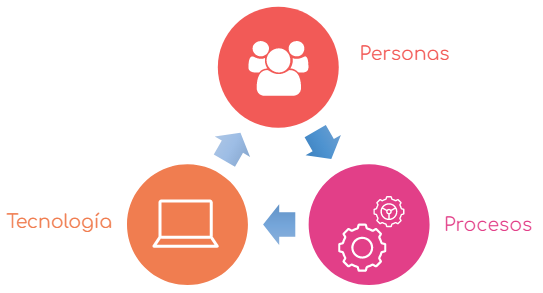
\includegraphics[width=0.7\textwidth]{imgs/1.png}
            \end{figure}
            
            \newpage
            
            \subsubsection*{¿Por qué es necesaria la calidad?}
            \addcontentsline{toc}{subsubsection}{¿Por qué es necesaria la calidad?}
            
            La experiencia nos dice que esta es esencial para \textbf{sobrevivir}, durante años milenios, las mejoras de calidad nos han permitido obtener mejor calidad de vida. Es esencial para \textbf{exportar}, para bajar \textbf{costos}, para aumentar el \textbf{valor} de lo ofrecido y con ello las utilidades. Sirve para \textbf{fidelizar} clientes y es un asunto de \textbf{competitividad}.
            
            \begin{figure}[h]
                \centering
                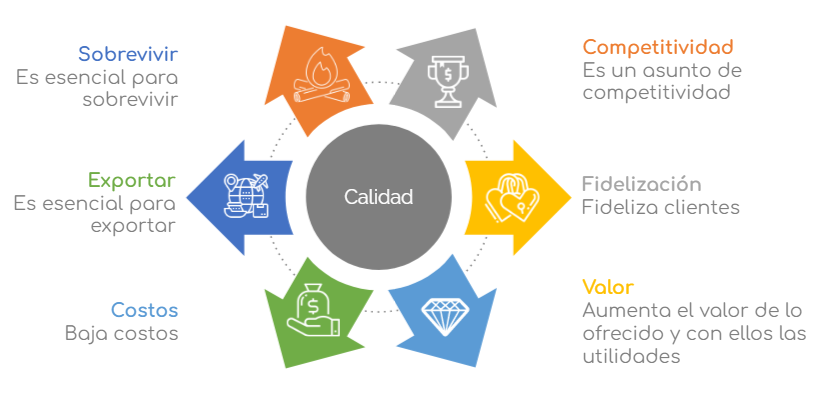
\includegraphics[width=\textwidth]{imgs/2.png}
            \end{figure}
            
            La calidad, productividad y los costos siempre van de la mano. En una organización de software, la calidad es proporcional a la productividad.
    \subsection*{Conceptos de testing de Software}
    
    
    \addcontentsline{toc}{subsection}{Conceptos de testing de Software}
    La calidad no puede ser lograda evaluando un producto que ya se encuentra completado. Por lo que el objetivo que tenemos que tener en mente es prevenir defectos o deficiencias en primer lugar y hacer que los productos sean evaluables mediante medidas de garantía de calidad. Algunas de estas incluyen estructurar el proceso de desarrollo con un estándar de desarrollo de software ya establecido. Y apoyar este con diferentes métodos técnicas y herramientas. Estos pueden incluir procedimientos para copia de seguridad de datos, metodología de prueba, gestión de cambios, documentación de defectos y reconciliación, documentación de estándares de codificación y prescripción y usos de estándares.
    
    La gestión de calidad disminuye los costos de producción, ya que entre antes se encuentre y corrija un defecto, menos costoso será a largo plazo. Con la aparición de las herramientas de prueba automatizadas, la inversión inicial puede llegar a ser sustancial, pero  el resultado a largo plazo serán productos de mayor calidad y con costos de mantenimiento reducidos.
    
    Los costos asociados a una gestión de calidad efectiva consisten en la suma de los costos de cuatro componentes: \textbf{prevención}, \textbf{inspección}, \textbf{falla interna} y \textbf{falla externa}.
    
    \begin{itemize}
        \item Los costos de prevención consisten en acciones tomadas para evitar que ocurran defectos en primer lugar.
        \item Los costos de inspección consisten en medir, evaluar y auditar productos o servicios para verificar el cumplimiento de las normas y especificaciones requeridas.
        \item Los costos de falla interna corresponden a aquellos incurridos en la reparación de productos defectuosos antes de ser entregados.
        \item Los costos de fallas externas son aquellos que aparecen al descubrir defectos después del lanzamiento del producto.
    \end{itemize}
    
    Esto último puede ser devastador, ya que puede dañar la reputación de la organización y/o provocar la pérdida de ventas futuras. La mayor recuperación de costos se realiza a través de la prevención. Aumentar el énfasis en ella reduce la cantidad de defectos que pasan al cliente sin ser detectados.
    
    \subsubsection*{Verificación}
    \addcontentsline{toc}{subsubsection}{Verificación}
    Consiste en:
        \begin{itemize}
            \item Asegurarse de que el software corresponda a los requisitos levantados.
            \item Confirmar que el producto corresponde con sus especificaciones.
            \item Demuestra que el producto se está haciendo como se dijo que se haría.
            \item Se puede realizar contrastando artefactos entre sí.
            \item \textit{¿Estamos resolviendo correctamente el problema?}
        \end{itemize}
    
    \subsubsection*{Validación}
    \addcontentsline{toc}{subsubsection}{Validación}
    
        \begin{itemize}
            \item Consiste en asegurarse de que los requisitos correspondan al problema. En comprobar que una aplicación sirve para el propósito por la que fue solicitada.
            \item Relacionada con posibles problemas en la especificación de requisitos
            \item Se enfoca en que el producto haga lo esperado.
            \item Se puede realizar contrastando un artefacto con la realidad
            \item \textit{¿Estamos resolviendo el problema correcto?}
        \end{itemize}
    
    \subsection*{Atributos de calidad}
    \addcontentsline{toc}{subsection}{Atributos de calidad}
    
    Un atributo de calidad es una propiedad medible de un sistema, que indica qué tan bien el sistema satisface las necesidades de las partes interesadas.
    
    Atributos de calidad de software comunes son:
    
    \begin{multicols}{2}
    \begin{itemize}
        \item Correcto
        \item Confiable
        \item Robusto
        \item Rendimiento
        \item Amigable
        \item Verificable
        \item Reusable
        \item Portable
        \item Elástico
        \item Estable
        \item Interoperable
        \item Productivo
        \item A tiempo
        \item Visible
        \item Cohesivo
        \item Desacoplado
        \item Comprensible
        \item Mantenible
    \end{itemize}
    \end{multicols}
    
    \subsubsection*{Correcto}
        Se comporta de acuerdo a su especificación. La definición supone la existencia de una especificación de requisitos y la posibilidad de determinar, sin ambigüedad, la correspondencia entre la especificación y la realización. La corrección del software puede comprobarse mediante pruebas o análisis.
        
    \subsubsection*{Confiable}

        Se comporta de acuerdo a lo esperado por el usuario. A diferencia de la corrección, la confiabilidad es algo relativo. El mercado puede admitir algunos errores en el software siempre que, en general, se comporte de forma esperable. No hay garantías de corrección del software, varios productos incluyen un \textit{disclaimer}.
    
    \subsubsection*{Robusto}

        Se comporta en forma razonable aún en situaciones no anticipadas. Datos de entrada incorrectos o fallas de hardware son situaciones más frecuentes. Si algo se especifica como requisito, cumplirlo es cuestión de corrección, de lo contrario, es cuestión de robustez. El esfuerzo dedicado a la robustez depende de la experiencia de los usuarios o lo crítico de su misión. 
    
    \subsubsection*{Rendimiento}

        Usa sus recursos en forma económica. Los criterios de rendimiento varían con la tecnología y el tiempo. De ser muy lento se reduce la productividad de los usuarios. Si utiliza mucha memoria del disco, puede afectar a otros sistemas. El rendimiento parte con la arquitectura. Métodos de evaluación de este son el análisis, el monitoreo y la simulación.
    
    \subsubsection*{Amigable}

        O usable, los usuarios lo encuentran fácil de usar. La interfaz del usuario es esencial. Para usuarios nuevos, lo mejor son largos mensajes explicativos, mientras que los usuarios expertos aprecian más los atajos. Los sistemas incrustados (\textit{embedded}) son amigables si son fáciles de configurar. Factores críticos para este atributo son la consistencia, el rendimiento y la confiabilidad.
    
    \subsubsection*{Verificable}

        sus propiedades pueden ser comprobadas. Aquí se interesan todas las propiedades: corrección, rendimiento, seguridad, etc. La verificación puede hacerse mediante análisis o pruebas. Software's más verificables poseen monitores en el código, tienen un diseño modular, sus desarrolladores poseen disciplina en la codificación y se utilizan el lenguaje de programación adecuado.
    
    \subsubsection*{Reusable}

        Se reutiliza a bajo costo. Este atributo es más aplicable a componentes que a sistemas complejos. Un ejemplo corresponde a las librerías o los frameworks con los que estamos muy familiarizados. El reuso es difícil de conseguir a posteriori.
    
    \subsubsection*{Portable}

        Puede ejecutarse en distintos ambientes (hardware, software, Sistemas operativos, etc). Una forma de lograr portabilidad es que esta suponga la mínima configuración posible, esto penaliza a los sistemas que podrían ejecutar mejor, haciendo uso del ambiente disponible. Otra opción es determinar, sobre la marcha, las disponibilidades del ambiente.
    
    \subsubsection*{Flexible, elástico, interoperable}

        Puede coexistir y cooperar con otros sistemas. Los componentes reutilizables son inherentemente interoperables. Las interfaces estándares promueven la interoperabilidad. Los sistemas abiertos son casos típicos de sistemas interoperables (como Unix).
    
    %\subsubsection*{Estable}
    %\addcontentsline{toc}{subsubsection}{Estable}
    
    \subsubsection*{Productivo}

        La productividad es la eficiencia del proceso de desarrollo del software. Es tamaño dividido por esfuerzo. La productividad de un equipo es distinta que la suma de productividades individuales. La automatización, el reuso y la buena calidad aumentan la productividad.
    
    \subsubsection*{A tiempo}

    U oportuno, el proceso de desarrollo debe obtener su producto en el tiempo planeado. Esto da una mejor oportunidad comercial y puede determinar la utilidad del producto. Aunque, tener un producto a tiempo sin confiabilidad o eficiencia, no es útil. Este atributo requiere estimación de trabajo, planificación con hitos verificables y gestión de riesgos.
    
    \subsubsection*{Visible}

    Un proyecto de software es visible si se puede saber el estado de su avance. La visibilidad ayuda a evaluar el impacto de las decisiones. También es esencial cuando existe rotación en el personal. El diseño, la codificación, las pruebas y la integración pueden ser en paralelo si están coordinadas.
    
    \subsubsection*{Cohesivo}

        Medida de la relación entre las partes de un sistema. Coincidental, no relacionados. Lógica, funciones similares. Temporal, ejecución simultánea. Procedural, secuencia de control. Comunicacional, comparten la entrada. Secuencial, salida de uno es entrada del otro. Funcional, todas las partes son necesarias para la función. Objeto, todas las acciones actúan sobre los mismos datos del objeto.
    
    \subsubsection*{Desacoplado o acoplado}

        Medida de la interdependencia de distintos componentes. Los sistemas muy acoplados compartes variables e información de control. Por otro lado, los desacoplados tienen interfaces definidas con listas de parámetros.
    
    \subsubsection*{Comprensible}

        Es fácil comprender cómo funciona. Nombres, documentación y complejidad afectan la comprensibilidad, así como qué tan cohesivo y acoplado es el sistema. Si un sistema es comprensible, es también, más mantenible y verificable. Desde el punto de vista del usuario, que un sistema sea más comprensible es que este sea amigable/usable y robusto.
    
    \subsubsection*{Mantenible}

        Es fácil de modificar y administrar en el tiempo. Que el software sea mantenible implica que es reparable, con facilidad para corregir defectos y es evolucionable, con facilidad para agregar funcionalidades. Existen tipos de mantenimiento, correctivo, para remover errores presentes en el software. Adaptativo, ajustar el software a cambios del entorno. Perfectivo, cambiar el software para mejorar alguna de sus cualidades.\\
    
    Para continuar con el curso, debemos ser consientes de las siguientes distinciones:
    
    \subsubsection*{Bug}

    Todos conocemos el concepto de \textit{bug}, pero debemos ser más profesionales, tenemos que conocer las distinciones y utilizar las palabras correctas para describir los problemas que estamos enfrentando:
    
    \subsubsection*{Error}

    Es una acción humana que tiene como desenlace un resultado incorrecto. Es una equivocación del desarrollador o del analista. Puede producirse por una idea falsa o equivocada. Un error puede llevarnos a generar defectos.
    
    Ejemplos:
    
    \begin{itemize}
        \item Error en la programación
        \item Error en el tipeo
        \item Requerimiento mal especificado o mal levantado
    \end{itemize}
    
    \subsubsection*{Defecto}

    Es un desperfecto en un componente que puede causar que el mismo falle en su funcionamiento. Es cualquier tipo de evento en un programa que hace que el sistema bajo prueba realice una de las siguientes acciones:
    
    \begin{enumerate}
        \item No cumplir con los requisitos especificados (funcionales o no funcionales)
        \item Devolver el resultado incorrecto
        \item Detener la ejecución inesperadamente
    \end{enumerate}
    
    Ejemplos:
    
    \begin{itemize}
        \item Sentencia o definición de datos incorrecta
        \item El desarrollador utilizó un operador que no corresponde
        \item \textbf{El sistema no cumple con los requisitos}
    \end{itemize}
    
    \subsubsection*{Falla}

    Es la manifestación visible de un defecto. Esta es producida por el error humano y por las condiciones ambientales:
    
    \begin{itemize}
        \item El defecto se introdujo en el código del software, en datos o parámetros de configuración
        \item Alguna condición física, como la temperatura, humedad, radiación o el suministro de electricidad la produjo.
    \end{itemize}
    
    Ejemplo:
    
    \begin{itemize}
        \item Un crash en el sistema durante la ejecución de una aplicación.
    \end{itemize}
    
    \subsubsection*{Relación y dependencias}

    \begin{figure}[h]
        \centering
        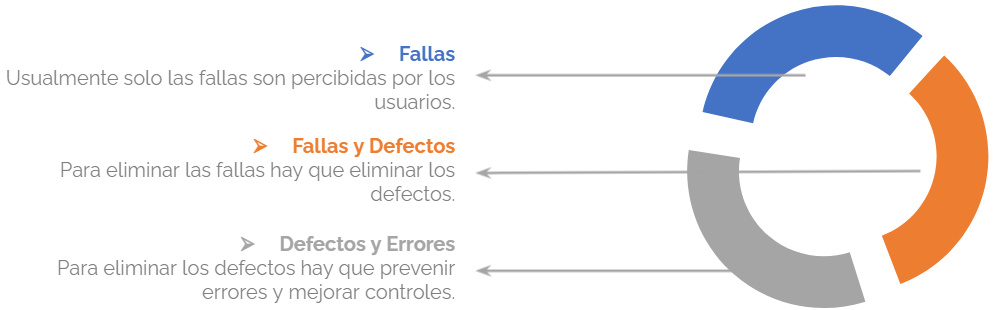
\includegraphics[width=0.7\textwidth]{imgs/3.png}
    \end{figure}
    
    \subsubsection*{Criterios de clasificación de defectos}

    
    Es conveniente clasificar los defectos para poder entender dónde nos equivocamos en mayor medida y así generar un esquema de mejora continua.
    
    \begin{itemize}
        \item ¿Dónde?: Detección de la fase del ciclo de vida en la que se produce el defecto
        \item ¿Cuándo?: Detección de la fase del ciclo de vida en la que se detecta el defecto
        \item Consecuencias: Gravedad del defecto, medida de las consecuencias que este produce en el sistema (Cosmético, menor; Sistema no disponible, bloqueante)
        \item Clasificación: Clasificación de problemas de codificación (Inicialización, definición de datos, referencia nula, interfaz, control de flujo, condición, sincronización, etc.)
        \item ¿Qué?: Carácter, acción u omisión.
    \end{itemize}
    
    %\subsection*{Escenario actual}
    \addcontentsline{toc}{subsection}{Escenario actual}
    %\subsection*{Rol del analista de calidad}
    \addcontentsline{toc}{subsection}{Rol del analista de calidad}
    %\subsection*{Rol del líder de calidad}
    \addcontentsline{toc}{subsection}{Rol del líder de calidad}
    
    %El acercamiento de Google es un poco contra-intuitivo, tienen menos personal dedicado principalmente al testing en toda la empresa, que la mayoría de sus competidores en uno solo de sus productos. Gracias a los pocos testers presentes, estos debieron mejorar cómo priorizaban lo que hacían. Desde características hasta técnicas de testeo, aprendieron a crear actividades con gran impacto y bajo arrastre  en su búsqueda por calidad. Entonces, ¿Cómo se las arregla Google con un grupo pequeño de personas de prueba? La calidad está puesta sobre los hombros de quienes escriben el código. Todos los programadores, son también probadores de sus códigos, la calidad es el problema de este colectivo. Si eres ingeniero, eres tester, si tu título posee la palabra prueba, entonces eres un facilitador de buenas pruebas. La cultura y la práctica de pruebas está centrada en el desarrollador. Si un producto falla, el primer punto de escalamiento es el desarrollador que pudo ser responsable de crear ese problema, no es quien estaba evaluando y no lo detectó. Lo anterior permite que la calidad sea un acto de prevención más que uno de detección. La calidad es un problema de desarrollo, no de pruebas.
    
    %Responsables de calidad. El gerente de pruebas es responsable de garantizar que un producto cumpla con un nivel aceptable de cumplimiento de los requisitos funcionales y no funcionales. Quienes son responsables por la calidad deben analizar los requerimientos, realizar un análisis de brecha (entre fases y componentes de estos), definir los datos de prueba y los medios para esta,validar el ambiente de pruebas, analizar los resultados de las pruebas, deben entregar calidad. Deben también encontrar errores importantes de forma rápida, deben proporcionar una evaluación general de la calidad del producto. Deben certificar que el producto cumple con el estándar definido, ayudar a sus clientes a mejorar la calidad y la capacidad de prueba del producto. Tienen que educar a estos sobre las pruebas y sobre cómo trabajar con el equipo de calidad. Deben ayudar a predecir y controlar los costos de soporto, además de ayudar a sus clientes a mejorar sus procesos. Su trabajo debe ser realizado de forma que el costo, los tiempos utilizados y los efectos secundarios indeseables se minimicen. Se debe hacer lo necesario para satisfacer a los clientes.
    
    %Consejos para los responsables de calidad. Pedir ayudas a otros cuando sea necesario. Los problemas deben ser comunicados en la medida en que surgen. Es importante actualizar siempre el conocimiento del negocio, aprender nuevas tecnologías y herramientas de prueba. Se debe mejorar el proceso y crear una base de conocimiento. Se debe evangelizar sobre la importancia del testing.